\section{Algebra of principal-minor extensions}\label{sec:minor-moves}

We now turn to Proposition~\ref{prop:path-potential}, which controls the
potential in expectation. We will grow nonsingular principal minors by one
or two coordinates.
The following deletion lemma supplies such moves in reverse order, with
the additional condition required when two coordinates must be deleted.

\begin{lemma}[Gated deletion]\label{lem:gated-deletion}
Let \(B\) be a nonsingular symmetric \(r\times r\) matrix with entries
in \(\bits\), where \(r\ge1\). Either a principal submatrix obtained by
deleting one coordinate is nonsingular, or there are distinct coordinates
\(i,j\) such that, with \(I=[r]\setminus\{i,j\}\),
\[
 C=B_{I,I}\quad\hbox{is nonsingular},\qquad
 v_1=B_{I,i}\in\mathcal S(C),\quad v_2=B_{I,j}\in\mathcal S(C).
\]
For the empty minor we use determinant one, and \(\mathcal S\) contains
its unique empty column.
\end{lemma}

\begin{proof}
The cofactor identity gives
\[
 \det B_{[r]\setminus\{i\},[r]\setminus\{i\}}
   =\det B\,(B^{-1})_{ii}.
\]
Thus a nonzero diagonal entry of \(B^{-1}\) gives the first alternative.
Suppose instead that all diagonal entries of \(B^{-1}\) vanish. Since
\(B^{-1}\) is nonsingular, it has a nonzero off-diagonal entry. Choose
\(i,j\) to maximize the absolute value of an entry of \(B^{-1}\), and
write \(\kappa=(B^{-1})_{ij}\ne0\). Then
\[
 (B^{-1})_{\{i,j\},\{i,j\}}=
 \begin{pmatrix}0&\kappa\\ \kappa&0\end{pmatrix}.
\]
Jacobi's complementary minor identity gives
\[
 \det C=\det B\,
          \det (B^{-1})_{\{i,j\},\{i,j\}}
        =-\kappa^2\det B\ne0.
\]

Order the coordinates with \(I\) first and write
\[
 B=\begin{pmatrix}C&V\\ V^{\mathsf T}&D\end{pmatrix},
 \qquad V=(v_1\ v_2),\qquad
 T=D-V^{\mathsf T}C^{-1}V.
\]
Block inversion shows that
\[
 T^{-1}=(B^{-1})_{\{i,j\},\{i,j\}}
       =\begin{pmatrix}0&\kappa\\ \kappa&0\end{pmatrix},
 \qquad
 (B^{-1})_{I,\{i,j\}}=-C^{-1}VT^{-1}.
\]
The diagonal of \(T\) is therefore zero. Its two diagonal equations give
\(v_a^{\mathsf T}C^{-1}v_a=D_{aa}\in\bits\) for \(a=1,2\). Moreover,
the two columns of the displayed inverse block are
\(-\kappa C^{-1}v_2\) and \(-\kappa C^{-1}v_1\). Every entry in that
block has absolute value at most \(|\kappa|\), by the choice of \(i,j\).
Hence \(\|C^{-1}v_a\|_\infty\le1\) for \(a=1,2\). These two facts are
exactly the defining conditions for \(v_1,v_2\in\mathcal S(C)\).
\end{proof}

For \(h\in\{1,2\}\), let \(m,m+h\in\mathcal I_N\), and let \(C\) be
a nonsingular binary matrix of size \(m\). A \emph{random extension of
width \(h\)} is
\begin{equation}\label{eq:random-extension}
 B=\begin{pmatrix}C&V\\ V^{\mathsf T}&D\end{pmatrix},
 \qquad V=(v_1\ \cdots\ v_h).
\end{equation}
The \(mh\) entries of \(V\) and the \(h(h+1)/2\) entries \(D_{ab}\),
\(1\le a\le b\le h\), are mutually independent uniform bits; the lower
triangle of \(D\) is determined by symmetry. If \(C\) is random, all
these new bits are also independent of \(C\). Thus, conditional on the
entire matrix \(C\), the columns \(v_1,\ldots,v_h\) are independent
uniform elements of \(\bits^m\), independent of all upper-triangular
entries of \(D\). Writing \(\Omega\) for this extension's sample space,
define the gate events by
\begin{equation}\label{eq:extension-gate}
 \mathcal G_1=\Omega,\qquad
 \mathcal G_2=\{v_1\in\mathcal S(C),\ v_2\in\mathcal S(C)\}.
\end{equation}
Conditional independence of the two columns gives
\begin{equation}\label{eq:gate-probability}
 \Pr(\mathcal G_2\mid C)=\left(\frac{|\mathcal S(C)|}{2^m}\right)^2.
\end{equation}
This identity lets the admissible-column estimate pay for the potential
bound on extensions of width two.
Lemma~\ref{lem:gated-deletion} shows that every nonsingular matrix has a
backward move whose forward extension satisfies its gate.

\begin{proposition}[Potential step]\label{prop:potential-step}
For every fixed \(A>0\), the following holds typically for nonsingular
binary matrices \(C\) of size \(m\in\mathcal I_N\). For each
\(h\in\{1,2\}\) with \(m+h\in\mathcal I_N\), the random extension
in Equation~\eqref{eq:random-extension} satisfies
\begin{equation}\label{eq:potential-step}
 \E\!\left[
   \ind_{\{\det B\ne0\}}\ind_{\mathcal G_h}\,2^{N\Psi(B)}
   \,\middle|\, C\right]
 \le 2^{N(\Psi(C)+\ell^{-A})}.
\end{equation}
The typical condition is imposed only on the starting matrix \(C\).
\end{proposition}

Proposition~\ref{prop:potential-step} will be proved in
Section~\ref{sec:potential-step}. We first establish the algebraic facts
that relate an extension to quotients of \(G_C\).

\subsection{The common quotient and its layers}

Fix a realization of Equation~\eqref{eq:random-extension} for which
\(B\) is nonsingular. Set
\begin{equation}\label{eq:successive-quotients}
 H_0=G_C,\qquad
 H_j=\Z^m/(C\Z^m+\Z v_1+\cdots+\Z v_j)
     =H_{j-1}/\langle\overline v_j\rangle
       \quad(1\le j\le h),
\end{equation}
where \(\overline v_j\) is the image of \(v_j\) in \(H_{j-1}\).
These finite groups depend only on \(C\) and the indicated columns.
They are defined whenever \(C\) is nonsingular, even if the destination
matrix \(B\) is singular. Nonsingularity of \(B\) is needed only when
we refer to its discriminant group.
The last one is also a quotient of \(G_B\):
\begin{equation}\label{eq:common-quotient}
 H_h\cong G_B/\langle\overline e_{m+1},\ldots,
                         \overline e_{m+h}\rangle,
\end{equation}
where the bars on the right denote classes of standard basis vectors in
\(G_B\). Indeed, the right side is
\[
 \Z^{m+h}/\bigl(B\Z^{m+h}+(0\oplus\Z^h)\bigr).
\]
Projection onto the first \(m\) coordinates maps its relations to
\(C\Z^m+V\Z^h\). Conversely, if a vector in \(\Z^{m+h}\) projects
into \(C\Z^m+V\Z^h\), subtracting a suitable vector of
\(B\Z^{m+h}\) leaves a vector in \(0\oplus\Z^h\). Projection
therefore induces exactly the isomorphism in
Equation~\eqref{eq:common-quotient}.

For a finite abelian group \(G\), a prime \(p\), and an integer
\(t\ge0\), define
\begin{equation}\label{eq:layer-prefix}
 F_G(p,t)=\sum_{e=1}^{t}k_G(p,e)
         =\sum_i\min\{b_{p,i},t\}
         =\log_p|G/p^tG|.
\end{equation}
The empty sum is zero. The two equalities follow directly from the
cyclic decomposition of the \(p\)-primary part; multiplication by
\(p^t\) is an automorphism on every other primary part. For a
nonsingular binary matrix \(M\), write \(F_M(p,t)=F_{G_M}(p,t)\).

\begin{lemma}[Layers under a one-element quotient]\label{lem:layer-quotient}
Let \(G\) be a finite abelian group, let \(v\in G\), and put
\(H=G/\langle v\rangle\). Fix a prime \(p\), and define \(u_t\) by
\[
 p^{u_t}=|\langle v+p^tG\rangle|\quad\hbox{in }G/p^tG
 \qquad(t\ge0).
\]
Then \(u_0=0\), \(u_t-u_{t-1}\in\{0,1\}\) for \(t\ge1\), and
\begin{align}
 F_H(p,t)&=F_G(p,t)-u_t,\label{eq:quotient-prefix}\\
 k_H(p,e)&=k_G(p,e)-(u_e-u_{e-1})\in
           \{k_G(p,e),k_G(p,e)-1\}.\label{eq:layer-interlacing}
\end{align}
Call a positive layer \((p,e)\) of \(G\) \emph{retained} if
\(k_H(p,e)=k_G(p,e)\). On every maximal interval of consecutive
layers where \(k_G(p,e)\) has a fixed positive value, the retained
layers form an initial interval, possibly empty. We call such an
interval of constant height a \emph{plateau}.
\end{lemma}

\begin{proof}
Quotienting by \(p^t\) and by \(v\) commutes:
\[
 H/p^tH\cong (G/p^tG)/\langle v+p^tG\rangle.
\]
Taking orders proves Equation~\eqref{eq:quotient-prefix}.

Write \(G_p=\bigoplus_i\Z/p^{b_i}\Z\). For the \(i\)-th coordinate
of the \(p\)-primary component of \(v\), let \(r_i\) be its
\(p\)-adic valuation capped at \(b_i\); in particular \(r_i=b_i\)
for a zero coordinate. The order of that coordinate in
\(G_p/p^tG_p\) is \(p^{(\min\{b_i,t\}-r_i)_+}\), where
\(x_+=\max\{x,0\}\). The order of an element in a direct sum of
\(p\)-groups is the largest of its coordinate orders, so
\begin{equation}\label{eq:quotient-order-exponent}
 u_t=\max_i(\min\{b_i,t\}-r_i)_+,
\end{equation}
with maximum zero when \(G_p\) is trivial. Each function under this
maximum is nondecreasing in \(t\) and increases by at most one at a
step. The same is therefore true of \(u_t\); since it is integer
valued, its increments belong to \(\{0,1\}\). Subtracting
Equation~\eqref{eq:quotient-prefix} at \(t=e-1\) from the equation at
\(t=e\) proves Equation~\eqref{eq:layer-interlacing}.

On a plateau of height \(k\), the heights in \(H\) are either \(k\)
or \(k-1\). They are nonincreasing as \(e\) increases, by their
definition from invariant factors. Thus a height \(k-1\) cannot be
followed on the plateau by height \(k\). The retained layers are
exactly those of height \(k\), proving the prefix assertion.
\end{proof}

\begin{figure}[H]
\centering
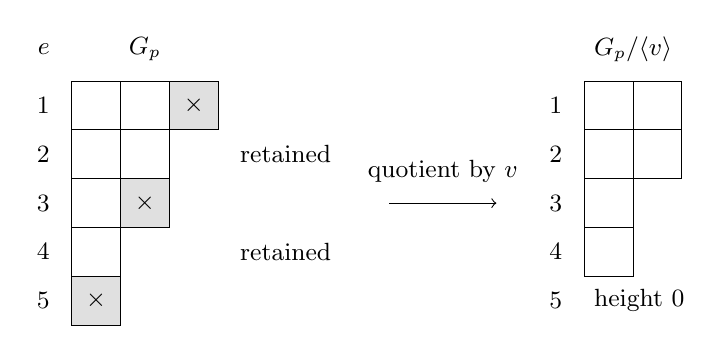
\begin{tikzpicture}[x=0.62cm,y=-0.62cm,
                    every node/.style={font=\small},
                    line width=0.4pt]
 \node at (1.5,-0.65) {\(G_p\)};
 \node[anchor=east] at (-0.25,-0.65) {\(e\)};
 \foreach \e/\k in {1/3,2/2,3/2,4/1,5/1} {
  \node[anchor=east] at (-0.25,{\e-0.5}) {\(\e\)};
  \foreach \i in {1,...,\k} {
   \draw ({\i-1},{\e-1}) rectangle (\i,\e);
  }
 }
 \foreach \e/\i in {1/3,3/2,5/1} {
  \draw[fill=black!12] ({\i-1},{\e-1}) rectangle (\i,\e);
  \node at ({\i-0.5},{\e-0.5}) {\(\times\)};
 }
 \node[anchor=west] at (3.25,1.5) {retained};
 \node[anchor=west] at (3.25,3.5) {retained};
 \draw[->] (6.5,2.5) -- (8.7,2.5);
 \node at (7.6,1.85) {quotient by \(v\)};
 \node at (11.5,-0.65) {\(G_p/\langle v\rangle\)};
 \foreach \e/\k in {1/2,2/2,3/1,4/1} {
  \node[anchor=east] at (10.25,{\e-0.5}) {\(\e\)};
  \foreach \i in {1,...,\k} {
   \draw ({\i+9.5},{\e-1}) rectangle ({\i+10.5},\e);
  }
 }
 \node[anchor=east] at (10.25,4.5) {\(5\)};
 \node[anchor=west] at (10.5,4.5) {height \(0\)};
\end{tikzpicture}

\caption{Layers for \(G_p=\Z/p^5\Z\oplus\Z/p^3\Z\oplus\Z/p\Z\)
and its quotient by \(v=(p^2,p,1)\). The crossed boxes are the layer
drops. Here \((u_1,\ldots,u_5)=(1,1,2,2,3)\), so the retained layers
are \(e=2,4\). On each plateau \(e=2,3\) and \(e=4,5\), retention is
a prefix. The row lengths on the right are the heights of the quotient.}
\label{fig:layers}
\end{figure}

Applied successively to Equation~\eqref{eq:successive-quotients}, this
lemma gives a drop of zero or one at each layer in each quotient. The
same statement applies to the \(h\) successive quotients of \(G_B\)
by the standard basis classes in Equation~\eqref{eq:common-quotient}.
Consequently, for every \((p,e)\),
\begin{equation}\label{eq:common-layer-interlacing}
 k_C(p,e)-h\le k_{H_h}(p,e)\le k_C(p,e),\qquad
 k_B(p,e)-h\le k_{H_h}(p,e)\le k_B(p,e).
\end{equation}
In particular, for \(h=1\) the common height is either \(k_C(p,e)\)
or \(k_C(p,e)-1\), while \(k_B(p,e)\) is either the common height or
one more. This also shows that a layer absent from \(G_C\) has height
at most \(h\) in \(G_B\).

\subsection{The lattice forced by retention}

The next lemma extracts from a set of retained layers a necessary
divisibility condition on the column, with an exact formula for its index.
The condition lies in an
intermediate lattice between \(C\Z^m\) and \(\Z^m\), including when
one preceding column has already been quotiented out.

\begin{lemma}[Retention lattice]\label{lem:retention-lattice}
Let \(C\) be a nonsingular binary matrix of size \(m\), and let
\(\pi:\Z^m\twoheadrightarrow H\) be a quotient map to a finite
abelian group such that \(C\Z^m\subseteq\ker\pi\). Let \(E\) be
any set of positive layers of \(H\). There is a lattice \(K_E\),
depending only on \(\pi,H,E\), with
\begin{equation}\label{eq:retention-lattice}
 C\Z^m\subseteq K_E\subseteq\Z^m,\qquad
 [\Z^m:K_E]=N^{Nq(E)},\qquad
 q(E)=\sum_{(p,e)\in E} k_H(p,e)\nu_p,
\end{equation}
such that the following implication holds for every \(v\in\Z^m\):
if every layer in \(E\) is retained in
\(H\longrightarrow H/\langle\pi(v)\rangle\), then \(v\in K_E\).
\end{lemma}

\begin{proof}
For each prime choose, once for the given group \(H\), cyclic
coordinates
\[
 H_p=\bigoplus_i\Z/p^{b_i}\Z.
\]
Put
\[
 a_{p,i}=\#\{e:(p,e)\in E,\ e\le b_i\},\qquad
 T_E=\bigoplus_{p,i}p^{a_{p,i}}(\Z/p^{b_i}\Z)\subseteq H,
 \qquad K_E=\pi^{-1}(T_E).
\]
Here \(0\le a_{p,i}\le b_i\), and the subgroup in the \((p,i)\)
coordinate consists of the classes divisible by \(p^{a_{p,i}}\).
The lattice \(K_E\) contains \(C\Z^m\). Its index is
\[
 [\Z^m:K_E]=[H:T_E]
 =\prod_{p,i}p^{a_{p,i}}
 =\prod_{(p,e)\in E}p^{k_H(p,e)}
 =N^{Nq(E)},
\]
where the penultimate equality counts a selected layer once for each
cyclic factor reaching it. This proves all assertions about the lattice
and its index.

It remains to prove the implication. Fix \(p,i\), and let \(r_i\) be
the capped valuation of the \(i\)-th coordinate of \(\pi(v)\), as in
the proof of Lemma~\ref{lem:layer-quotient}. Equation~\eqref{eq:quotient-order-exponent}
at \(t=b_i\) gives \(u_{b_i}\ge b_i-r_i\). All the first \(b_i\)
layers are positive, and Equation~\eqref{eq:layer-interlacing} shows
that the number among them that are retained is
\[
 \sum_{e=1}^{b_i}\bigl(1-(u_e-u_{e-1})\bigr)=b_i-u_{b_i}.
\]
If every layer in \(E\) is retained, then
\[
 a_{p,i}\le b_i-u_{b_i}\le r_i.
\]
Thus the coordinate of \(\pi(v)\) is divisible by \(p^{a_{p,i}}\).
This holds in every primary coordinate, so \(\pi(v)\in T_E\) and
\(v\in K_E\), as required.
\end{proof}

For the group in Figure~\ref{fig:layers}, choosing
\(E=\{(p,2),(p,4)\}\) gives divisibility exponents
\((a_{p,1},a_{p,2},a_{p,3})=(2,1,0)\). The two selected layers have
total weight \(2\nu_p\), while \(q(E)=3\nu_p\) and
\([\Z^m:K_E]=p^3\).

For a quotient in Equation~\eqref{eq:successive-quotients}, the map
\(\pi\) is the natural map from \(\Z^m\) onto \(H_{j-1}\).
Conditional on \(C\) and the preceding columns
\(v_1,\ldots,v_{j-1}\), the next column remains uniform on the cube.

\subsection{A symmetric kernel inequality}

The common quotient also controls the destination layers more strongly
than interlacing alone. At a fixed prime \(p\), let \(u_{j,t}\) denote
the exponent from Lemma~\ref{lem:layer-quotient} for
\(H_{j-1}\to H_j\), and set
\begin{equation}\label{eq:total-quotient-loss}
 U_t=\sum_{j=1}^h u_{j,t}
    =F_C(p,t)-F_{H_h}(p,t).
\end{equation}
The equality follows by summing Equation~\eqref{eq:quotient-prefix}.

\begin{lemma}[Symmetric kernel inequality]\label{lem:layer-inequality}
For a nonsingular extension \(B\) of a nonsingular \(C\) of width
\(h\in\{1,2\}\), at every prime \(p\) and every integer \(t\ge0\),
\begin{equation}\label{eq:layer-inequality}
 F_B(p,t)\le F_C(p,t)+ht-2U_t.
\end{equation}
\end{lemma}

\begin{proof}
The assertion is immediate for \(t=0\). Fix \(t\ge1\), put
\(R_t=\Z/p^t\Z\), and reduce the blocks of \(B\) modulo \(p^t\),
writing them as \(C_t,V_t,D_t\). Let
\[
 X=R_t^m,\qquad Y=R_t^h,\qquad
 L=\ker(C_t:X\to X),\qquad J=\im(C_t:X\to X).
\]
The presentation of the cokernel gives
\[
 X/J\cong \Z^m/(C\Z^m+p^t\Z^m)\cong G_C/p^tG_C.
\]
Since \(C_t\) is an endomorphism of the finite group \(X\), its
kernel and cokernel have the same order. Hence
\begin{equation}\label{eq:kernel-prefix-order}
 |L|=|X/J|=p^{F_C(p,t)}.
\end{equation}

Define
\[
 \alpha:Y\longrightarrow X/J,\qquad \alpha(y)=V_ty+J.
\]
The image is the subgroup generated by the column classes in
\(G_C/p^tG_C\). Quotienting by that subgroup gives
\(H_h/p^tH_h\), so Equation~\eqref{eq:total-quotient-loss} gives
\[
 |\im\alpha|=p^{U_t},\qquad |\ker\alpha|=p^{ht-U_t}.
\]
For a kernel vector \((x,y)\in X\oplus Y\) of \(B\) modulo \(p^t\),
the first block equation is
\begin{equation}\label{eq:first-block-kernel}
 C_tx+V_ty=0.
\end{equation}
It requires \(y\in\ker\alpha\). For each such \(y\), its solutions
in \(x\) form a coset \(x_0+L\).

Consider the map
\[
 \gamma:L\longrightarrow Y,\qquad \gamma(z)=V_t^{\mathsf T}z.
\]
We claim that \(|\im\gamma|=p^{U_t}\). Equip \(X\) and \(Y\) with
their standard character pairings, for example
\[
 \langle x,z\rangle_X
   =\exp\!\left(\frac{2\pi i}{p^t}x^{\mathsf T}z\right).
\]
These pairings are perfect: a nonzero coordinate is detected by pairing
with its standard basis vector. For a subgroup \(M\) of either module
\(A\), write \(M^\perp\) for its annihilator. Character orthogonality
gives
\begin{equation}\label{eq:annihilator-order}
 |M|\,|M^\perp|
 =\sum_{a\in A}\sum_{z\in M}\langle a,z\rangle_A
 =|A|.
\end{equation}
For the first equality, the sum over \(M\) is \(|M|\) on its
annihilator and zero elsewhere. For the second, reverse the sums: by
perfectness the sum over \(A\) vanishes for every \(z\ne0\), and the
term \(z=0\) equals \(|A|\).

Symmetry of \(C_t\) gives \(J\subseteq L^\perp\), since
\(\langle C_tx,z\rangle_X=\langle x,C_tz\rangle_X=1\) for
\(z\in L\). Both groups have order \(|X|/|L|\), the former by the
kernel-image formula and the latter by
Equation~\eqref{eq:annihilator-order}. Therefore \(L^\perp=J\).
It follows that
\begin{align*}
 (\im\gamma)^\perp
  &=\{y\in Y:\langle y,V_t^{\mathsf T}z\rangle_Y=1
                    \text{ for every }z\in L\}\\
  &=\{y\in Y:\langle V_ty,z\rangle_X=1
                    \text{ for every }z\in L\}\\
  &=\{y\in Y:V_ty\in J\}=\ker\alpha.
\end{align*}
Equation~\eqref{eq:annihilator-order} in \(Y\) now gives
\[
 |\im\gamma|=\frac{|Y|}{|\ker\alpha|}=p^{U_t},
 \qquad
 |\ker\gamma|=\frac{|L|}{|\im\gamma|}
              =p^{F_C(p,t)-U_t}.
\]

For a fixed \(y\in\ker\alpha\) and \(x=x_0+z\) from
Equation~\eqref{eq:first-block-kernel}, the second block equation is
\[
 \gamma(z)=-V_t^{\mathsf T}x_0-D_ty.
\]
It has either no solutions or one coset of \(\ker\gamma\).
There are at most \(p^{ht-U_t}\) choices for \(y\), and for each at
most \(p^{F_C(p,t)-U_t}\) choices for \(z\). Consequently
\[
 |\ker(B\bmod p^t)|\le p^{F_C(p,t)+ht-2U_t}.
\]
As for \(C_t\), the kernel of the square endomorphism \(B\bmod p^t\)
has the same order as its cokernel. That cokernel is
\(G_B/p^tG_B\), of order \(p^{F_B(p,t)}\). Taking logarithms proves
Equation~\eqref{eq:layer-inequality}.
\end{proof}

Lemma~\ref{lem:retention-lattice} identifies the intermediate lattices
that arise from retaining layers, while Lemma~\ref{lem:layer-inequality}
uses symmetry to relate those retentions to the destination group.
Section~\ref{sec:cube} supplies a uniform bound on cube
intersections with every lattice of the form in
Equation~\eqref{eq:retention-lattice}.
